%%%%%%%%%%%%%%%%%%%% author.tex %%%%%%%%%%%%%%%%%%%%%%%%%%%%%%%%%%%
%
% sample root file for your "contribution" to a contributed volume
%
% Use this file as a template for your own input.
%
%%%%%%%%%%%%%%%% Springer %%%%%%%%%%%%%%%%%%%%%%%%%%%%%%%%%%


% RECOMMENDED %%%%%%%%%%%%%%%%%%%%%%%%%%%%%%%%%%%%%%%%%%%%%%%%%%%
\documentclass[graybox]{svmult}

% choose options for [] as required from the list
% in the Reference Guide

\usepackage{mathptmx}       % selects Times Roman as basic font
\usepackage{helvet}         % selects Helvetica as sans-serif font
\usepackage{courier}        % selects Courier as typewriter font
\usepackage{type1cm}        % activate if the above 3 fonts are
                            % not available on your system
%
\usepackage{makeidx}         % allows index generation
\usepackage{graphicx}        % standard LaTeX graphics tool
                             % when including figure files
\usepackage{multicol}        % used for the two-column index
\usepackage[bottom]{footmisc}% places footnotes at page bottom
\usepackage{subcaption} %% ADDED
%%% Personal packages
%\usepackage[utf8]{inputenc}

% see the list of further useful packages
% in the Reference Guide

\makeindex             % used for the subject index
                       % please use the style svind.ist with
                       % your makeindex program

%%%%%%%%%%%%%%%%%%%%%%%%%%%%%%%%%%%%%%%%%%%%%%%%%%%%%%%%%%%%%%%%%%%%%%%%%%%%%%%%%%%%%%%%%

\begin{document}
\tableofcontents

\title*{non-protein-coding RNAs as regulators of development in tunicates}
% Use \titlerunning{Short Title} for an abbreviated version of
% your contribution title if the original one is too long
\author{Author A and Author B}
% Use \authorrunning{Short Title} for an abbreviated version of
% your contribution title if the original one is too long
\institute{Author Name \at Name, Address of Institute, \email{writeemail@unal.edu.co}
\and   Author Name \at Name, Address of Institute \email{writeemail@com}}
%
% Use the package "url.sty" to avoid
% problems with special characters
% used in your e-mail or web address
%
\maketitle

\abstract*{Each chapter should be preceded by an abstract (10--15 lines long) that summarizes the content. The abstract will appear \textit{online} at \url{www.SpringerLink.com} and be available with unrestricted access. This allows unregistered users to read the abstract as a teaser for the complete chapter. As a general rule the abstracts will not appear in the printed version of your book unless it is the style of your particular book or that of the series to which your book belongs.
Please use the 'starred' version of the new Springer \texttt{abstract} command for typesetting the text of the online abstracts (cf. source file of this chapter template \texttt{abstract}) and include them with the source files of your manuscript. Use the plain \texttt{abstract} command if the abstract is also to appear in the printed version of the book.}

\abstract{Each chapter should be preceded by an abstract (10--15 lines long) that summarizes the content. The abstract will appear \textit{online} at \url{www.SpringerLink.com} and be available with unrestricted access. This allows unregistered users to read the abstract as a teaser for the complete chapter. As a general rule the abstracts will not appear in the printed version of your book unless it is the style of your particular book or that of the series to which your book belongs.\newline\indent
Please use the 'starred' version of the new Springer \texttt{abstract} command for typesetting the text of the online abstracts (cf. source file of this chapter template \texttt{abstract}) and include them with the source files of your manuscript. Use the plain \texttt{abstract} command if the abstract is also to appear in the printed version of the book.}



\section{Introduction}
\label{sec:1}

noncoding RNAs rols in tunicates development date earliest in the 90´s from the works of Swalla \& Jeffry in which RNAs localized in the yellow crescent or myoplasm, a cytoskeletal domain in oocytes of the ascidian \textit{Styela clava} were discovered \cite{Swalla1995}. This  yellow crescent or YC RNA identified to be present throughout embryonic development was the first example involved in envisioning the future of a growing family of ncRNAs that would play important roles in growth and development in tunicates\cite{Swalla1995}.

This asymmetrically distributed ascidian RNAs were part of the set of many other RNAs known as maternally synthesized cytoplasmically localized RNAs, discovered first in oocytes of Xenopus \cite{Bashirullah1998}

\section{miRNA families origin and evolutionary perspective}
\label{sec:2}

\subsection{miRNA identification and validation}
\subsubsection{Pasquinatelli2000.pdf}
\cite{Pasquinelli2000}
\textit{Two small RNAs regulate the timing of Caenorhabditis elegans development. Transition from the first to the second larval stage fates requires the 22-nucleotide lin-4 RNA, and transition from late larval to adult cell fates requires the 21-nucleotide let-7 RNA. The lin-4 and let-7 RNA genes are not homologous to each other, but are each complementary to sequences in the 3' untranslated regions of a set of protein-coding target genes that are normally negatively regulated by the RNAs. Here we have detected let-7 RNAs of approximately 21 nucleotides in samples from a wide range of animal species, including vertebrate, ascidian, hemichordate, mollusc, annelid and arthropod, but not in RNAs from several cnidarian and poriferan species, Saccharomyces cerevisiae, Escherichia coli or Arabidopsis. We did not detect lin-4 RNA in these species. We found that let-7 temporal regulation is also conserved: let-7 RNA expression is first detected at late larval stages in C. elegans and Drosophila, at 48 hours after fertilization in zebrafish, and in adult stages of annelids and molluscs. The let-7 regulatory RNA may control late temporal transitions during development across animal phylogeny.}

\subsubsection{Legendere2004.pdf}
\cite{Legendre2005}
\textit{MOTIVATION: MicroRNAs (miRNA) are essential 21-22 nt regulatory RNAs produced from larger hairpin-like precursors. Local sequence alignment tools such as BLAST are able to identify new members of known miRNA families, but not all of them. We set out to estimate how many new miRNAs could be recovered using a profile-based strategy such as that implemented in the ERPIN program. RESULTS: We constructed alignments for 18 miRNA families and performed ERPIN searches on animal genomes. Results were compared to those of a WU-BLAST search at the same E-value cutoff. The two combined approaches produced 265 new miRNA candidates that were not found in miRNA databases. About 17{\%} of hits were ERPIN specific. They showed better structural characteristics than BLAST-specific hits and included interesting candidates such as members of the miR-17 cluster in Tetraodon. Profile-based RNA detection will be an important complement of similarity search programs in the completion of miRNA collections.}

\subsubsection{Satdler2005.pdf}
\cite{Missal2005} 
\textit{The analysis of animal genomes showed that only a minute part of their DNA codes for proteins. Recent experimental results agree, however, that a large fraction of these genomes are transcribed and hence are probably functional at the RNA level. A computational survey of vertebrate genomes has predicted thousands of previously unknown ncRNAs with evolutionarily conserved secondary structures. Extending these comparative studies beyond vertebrates is difficult, however, since most ncRNAs evolve quickly at the sequence level while conserving their characteristic secondarystructures. RESULTS: We report on a computational screen of structured ncRNAs in the urochordate lineage based on a comparison of the genomic data from Ciona intestinalis, Ciona savignyi and Oikopleura dioica. We predict {\textgreater}1000 ncRNAs with an evolutionarily conserved RNA secondary structure. Of these, about a quarter are located in introns of known protein coding sequences. A few RNA motifs can be identified as known RNAs, including approximately 300 tRNAs, some 100 snRNA genes and a few microRNAs and snoRNAs}

\subsubsection{Stadler2007.pdf}
\cite{Will2007}
\textit{The RFAM database defines families of ncRNAs by means of sequence similarities that are sufficient to establish homology. In some cases, such as microRNAs and box H/ACA snoRNAs, functional commonalities define classes of RNAs that are characterized by structural similarities, and typically consist of multiple RNA families. Recent advances in high-throughput transcriptomics and comparative genomics have produced very large sets of putative noncoding RNAs and regulatory RNA signals. For many of them, evidence for stabilizing selection acting on their secondary structures has been derived, and at least approximate models of their structures have been computed. The overwhelming majority of these hypothetical RNAs cannot be assigned to established families or classes. We present here a structure-based clustering approach that is capable of extracting putative RNA classes from genome-wide surveys for structured RNAs. The LocARNA (local alignment of RNA) tool implements a novel variant of the Sankoff algorithm that is sufficiently fast to deal with several thousand candidate sequences. The method is also robust against false positive predictions, i.e., a contamination of the input data with unstructured or nonconserved sequences. We have successfully tested the LocARNA-based clustering approach on the sequences of the RFAM-seed alignments. Furthermore, we have applied it to a previously published set of 3,332 predicted structured elements in the Ciona intestinalis genome (Missal K, Rose D, Stadler PF (2005) Noncoding RNAs in Ciona intestinalis. Bioinformatics 21 (Supplement 2): i77-i78). In addition to recovering, e.g., tRNAs as a structure-based class, the method identifies several RNA families, including microRNA and snoRNA candidates, and suggests several novel classes of ncRNAs for which to date no representative has been experimentally characterized.}

\subsubsection{Norden-Krichmaretal2007.pdf}
\cite{Norden-Krichmar2007}
\textit{BACKGROUND: This study reports the first collection of validated microRNA genes in the sea squirt, Ciona intestinalis. MicroRNAs are processed from hairpin precursors to {\~{}}22 nucleotide RNAs that base pair to target mRNAs and inhibit expression. As a member of the subphylum Urochordata (Tunicata) whose larval form has a notochord, the sea squirt is situated at the emergence of vertebrates, and therefore may provide information about the evolution of molecular regulators of early development.RESULTS: In this study, computational methods were used to predict 14 microRNA gene families in Ciona intestinalis. The microRNA prediction algorithm utilizes configurable microRNA sequence conservation and stem-loop specificity parameters, grouping by miRNA family, and phylogenetic conservation to the related species, Ciona savignyi. The expression for 8, out of 9 attempted, of the putative microRNAs in the adult tissue of Ciona intestinalis was validated by Northern blot analyses. Additionally, a target prediction algorithm was implemented, which identified a high confidence list of 240 potential target genes. Over half of the predicted targets can be grouped into the gene ontology categories of metabolism, transport, regulation of transcription, and cell signaling.CONCLUSION: The computational techniques implemented in this study can be applied to other organisms and serve to increase the understanding of the origins of non-coding RNAs, embryological and cellular developmental pathways, and the mechanisms for microRNA-controlled gene regulatory networks.}
\subsubsection{Fuetal2008.pdf}
\cite{Fu2008}
\textit{Recent studies reveal correlation between microRNA (miRNA) innovation and increased developmental complexity. This is exemplified by dramatic expansion of the miRNA inventory in vertebrates, a lineage where genome duplication has played a significant evolutionary role. Urochordates, the closest extant group to the vertebrates, exhibit an opposite trend to genome and morphological simplification. We show that the urochordate, larvacean, Oikopleura dioica, possesses the requisite miRNA biogenic machinery. The miRNAs isolated by small RNA cloning were expressed throughout the short life cycle, a number of which were stocked as maternal determinants prior to rapid embryonic development. We identify sex-specific miRNAs that appeared as male/female gonad differentiation became apparent and were maintained throughout spermatogenesis. Whereas 80{\%} of mammalian miRNAs are hosted in introns of protein-coding genes, the majority of O. dioica miRNA loci were located in antisense orientations to such genes. Including sister group ascidians in analysis of the urochordate miRNA repertoire, we find that 11 highly conserved bilaterian miRNA families have been lost or derived to the point they are not recognizable in urochordates and a further 4 of these families are absent in larvaceans. Subsequent to this loss/derivation, at least 29 novel miRNA families have been acquired in larvaceans. This suggests a profound reorganization of the miRNA repertoire integral to evolution in the urochordate lineage.}
\subsubsection{Hendrixetal2010.pdf}
\cite{Hendrix2010}
\textit{MicroRNAs (miRs) have been broadly implicated in animal development and disease. We developed a novel computational strategy for the systematic, whole-genome identification of miRs from high throughput sequencing information. This method, miRTRAP, incorporates the mechanisms of miR biogenesis and includes additional criteria regarding the prevalence and quality of small RNAs arising from the antisense strand and neighboring loci. This program was applied to the simple chordate Ciona intestinalis and identified nearly 400 putative miR loci.}

\subsubsection{Keshavanetal2010.pdf}

\cite{Keshavan2010}
MicroRNAs (miRNAs) are conserved non-coding small RNAs with potent post-transcriptional gene
regulatory functions. Recent computational approaches and sequencing of small RNAs had indicated
the existence of about 80 Ciona intestinalis miRNAs, although it was not clear whether other
miRNA genes were present in the genome. We undertook an alternative computational approach
to look for Ciona miRNAs. Conserved non-coding sequences from the C. intestinalis genome were
extracted and computationally folded to identify putative hairpin-like structures. After applying additional
criteria, we obtained 458 miRNA candidates whose sequences were used to design a custom
microarray. Over 100 of our predicted hairpins were identified in this array when probed with RNA
from various Ciona stages. We also compared our predictions to recently deposited sequences of
Ciona small RNAs and report that 170 of our predicted hairpins are represented in this data set.
Altogether, about 250 of our 458 predicted miRNAs were represented in either our array data or the
small-RNA sequence database. These results suggest that Ciona has a large number of genomically
encoded miRNAs that play an important role in modulating gene activity in developing
embryos and adults.


\subsubsection{Friedlander-2012.pdf}
\cite{Friedlander2012}
\textit{microRNAs (miRNAs) are a large class of small non-coding RNAs which post-transcriptionally regulate the expression of a large fraction of all animal genes and are important in a wide range of biological processes. Recent advances in high-throughput sequencing allow miRNA detection at unprecedented sensitivity, but the computational task of accurately identifying the miRNAs in the background of sequenced RNAs remains challenging. For this purpose, we have designed miRDeep2, a substantially improved algorithm which identifies canonical and non-canonical miRNAs such as those derived from transposable elements and informs on high-confidence candidates that are detected in multiple independent samples. Analyzing data from seven animal species representing the major animal clades, miRDeep2 identified miRNAs with an accuracy of 98.6-99.9{\%} and reported hundreds of novel miRNAs. To test the accuracy of miRDeep2, we knocked down the miRNA biogenesis pathway in a human cell line and sequenced small RNAs before and after. The vast majority of the {\textgreater}100 novel miRNAs expressed in this cell line were indeed specifically downregulated, validating most miRDeep2 predictions. Last, a new miRNA expression profiling routine, low time and memory usage and user-friendly interactive graphic output can make miRDeep2 useful to a wide range of researchers.}

\subsubsection{Teraietal2012.PDF}
\cite{Terai2012}
\textit{MicroRNA (miRNA) precursor hairpins have a unique secondary structure, nucleotide length, and nucleotide content that are in most cases evolutionarily conserved. The aim of this study was to utilize position-specific features of miRNA hairpins to improve their identification. To this end, we defined the evolutionary and structurally conserved features in each position of miRNA hairpins with heuristically derived values, which were successfully integrated using a probabilistic framework. Our method, miRRim2, can not only accurately detect miRNA hairpins, but infer the location of a mature miRNA sequence. To evaluate the accuracy of miRRim2, we designed a cross validation test in which the whole human genome was used for evaluation. miRRim2 could more accurately detect miRNA hairpins than the other computational predictions that had been performed on the human genome, and detect the position of the 5'-end of mature miRNAs with sensitivity and positive predictive value (PPV) above 0.4. To further evaluate miRRim2 on independent data, we applied it to the Ciona intestinalis genome. Our method detected 47 known miRNA hairpins among top 115 candidates, and pinpointed the 5'-end of mature miRNAs with sensitivity and PPV about 0.4. When our results were compared with deep-sequencing reads of small RNA libraries from Ciona intestinalis cells, we found several candidates in which the predicted mature miRNAs were in good accordance with deep-sequencing results.}


\subsubsection{Kusakabeetal2013.pdf}

\cite{Kusakabe2013}
\textit{Muscle-specific miR-1/206 and miR-133 families have been suggested to play fundamental roles in skeletal and cardiac myogenesis in vertebrates. To gain insights into the relationships between the divergence of these miRs and muscular tissue types, we investigated the expression patterns of miR-1 and miR-133 in two ascidian Ciona species and compared their genomic structures with those of other chordates. We found that Ciona intestinalis and Ciona savignyi each possess a single copy of the miR-1/miR-133 cluster, which is only 350 nucleotide long. During embryogenesis, Ciona miR-1 and miR-133 are generated as a single continuous primary transcript accumulated in the nuclei of the tail muscle cells, starting at the gastrula stage. In adults, mature miR-133 and miR-1 are differentially expressed in the heart and body wall muscle. Expression of the reporter gene linked to the 850-bp upstream region of the predicted transcription start site confirmed that this region drives the muscle-specific expression of the primary transcript of miR-1/miR-133. In many deuterostome lineages, including that of Ciona, the miR-1/133 cluster is located in the same intron of the mind bomb (mib) gene in reverse orientation. Our results suggest that the origin of genomic organization and muscle-specific regulation of miR-1/133 can be traced back to the ancestor of chordates. Duplication of this miR cluster might have led to the remarkable elaboration in the morphology and function of skeletal muscles in the vertebrate lineage. {\textcopyright} 2012 Elsevier B.V. All rights reserved.}

\subsubsection{Jueetal2016.pdf}
\cite{Jue2016}
\textit{A preliminary genome sequence has been assembled for the Southern Ocean salp, Salpa thompsoni (Urochordata, Thaliacea). Despite the ecological importance of this species in Antarctic pelagic food webs and its potential role as an indicator of changing Southern Ocean ecosystems in response to climate change, no genomic resources are available for S. thompsoni or any closely-related urochordate species. Using a multiple-platform, multiple-individual approach, we have produced a 318,767,936 bp genome sequence, covering more than 50{\%} of the estimated 602 MB (±173 MB) genome size for S. thompsoni Using a non-redundant set of predicted proteins, more than 50{\%} (16,823) of sequences showed significant homology to known proteins and {\~{}}38{\%} (12,151) of the total protein predictions were associated with Gene Ontology functional information. We have generated 109,958 SNP variant and 9,782 indel predictions for this species, serving as a resource for future phylogenomic and population genetic studies. Comparing the salp genome to available assemblies for four other urochordates, Botryllus schlosseri, Ciona intestinalis, Ciona savignyi and Oikopleura dioica, we found that S. thompsoni shares the previously-estimated rapid rates of evolution for these species. High mutation rates are thus independent of genome size, suggesting that rates of evolution {\textgreater}1.5 times that observed for vertebrates are a broad taxonomic characteristic of urochordates. Tests for positive selection implemented in PAML revealed a small number of genes with sites undergoing rapid evolution, including genes involved in ribosome biogenesis and metabolic and immune process that may be reflective of both adaptation to polar, planktonic environments as well as the complex life history of the salps. Finally, we performed an initial survey of small RNAs, revealing the presence of known, conserved miRNAs, as well as novel miRNA genes; unique piRNAs; and mature miRNA signatures for varying developmental stages. Collectively, these resources provide a genomic foundation supporting S. thompsoni as a model species for further examination of the exceptional rates and patterns of genomic evolution shown by urochordates. Additionally, genomic data will allow for the development of molecular indicators of key life history events and processes and afford new understandings and predictions of impacts of climate change on this key species of Antarctic pelagic ecosystems.}


\subsubsection{Wangetal2017.pdf}
\cite{Wang2017}
\textit{Background: miRNAs play essential roles in the modulation of cellular functions via degradation and/or translation
attenuation of target mRNAs. They have been surveyed in a single ascidian genus, Ciona. Recently, an annotated
draft genome sequence for a distantly related ascidian, Halocynthia roretzi, has become available, but miRNAs in
H. roretzi have not been previously studied.
Results: We report the prediction of 319 candidate H. roretzi miRNAs, obtained through three complementary
methods. Experimental validation suggests that more than half of these candidate miRNAs are expressed during
embryogenesis. The majority of predicted H. roretzi miRNAs appear specific to ascidians or tunicates, and only 32
candidates, belonging to 25 families, are widely conserved across metazoans.
Conclusion: Our study presents a comprehensive identification of candidate H. roretzi miRNAs. This resource
will facilitate the study of the mechanisms for miRNA-controlled gene regulatory networks during ascidian
development. Further, our analysis suggests that the majority of Halocynthia miRNAs are specific to ascidian
or tunicates, with only a small number of widely conserved miRNAs. This result is consistent with the general
notion that animal miRNAs are less conserved between taxa than plant ones.}



\subsection{miRNA in clusters}

\begin{figure}[ht!]
\centering
    \begin{subfigure}[t]{1.0\textwidth}
        \centering
        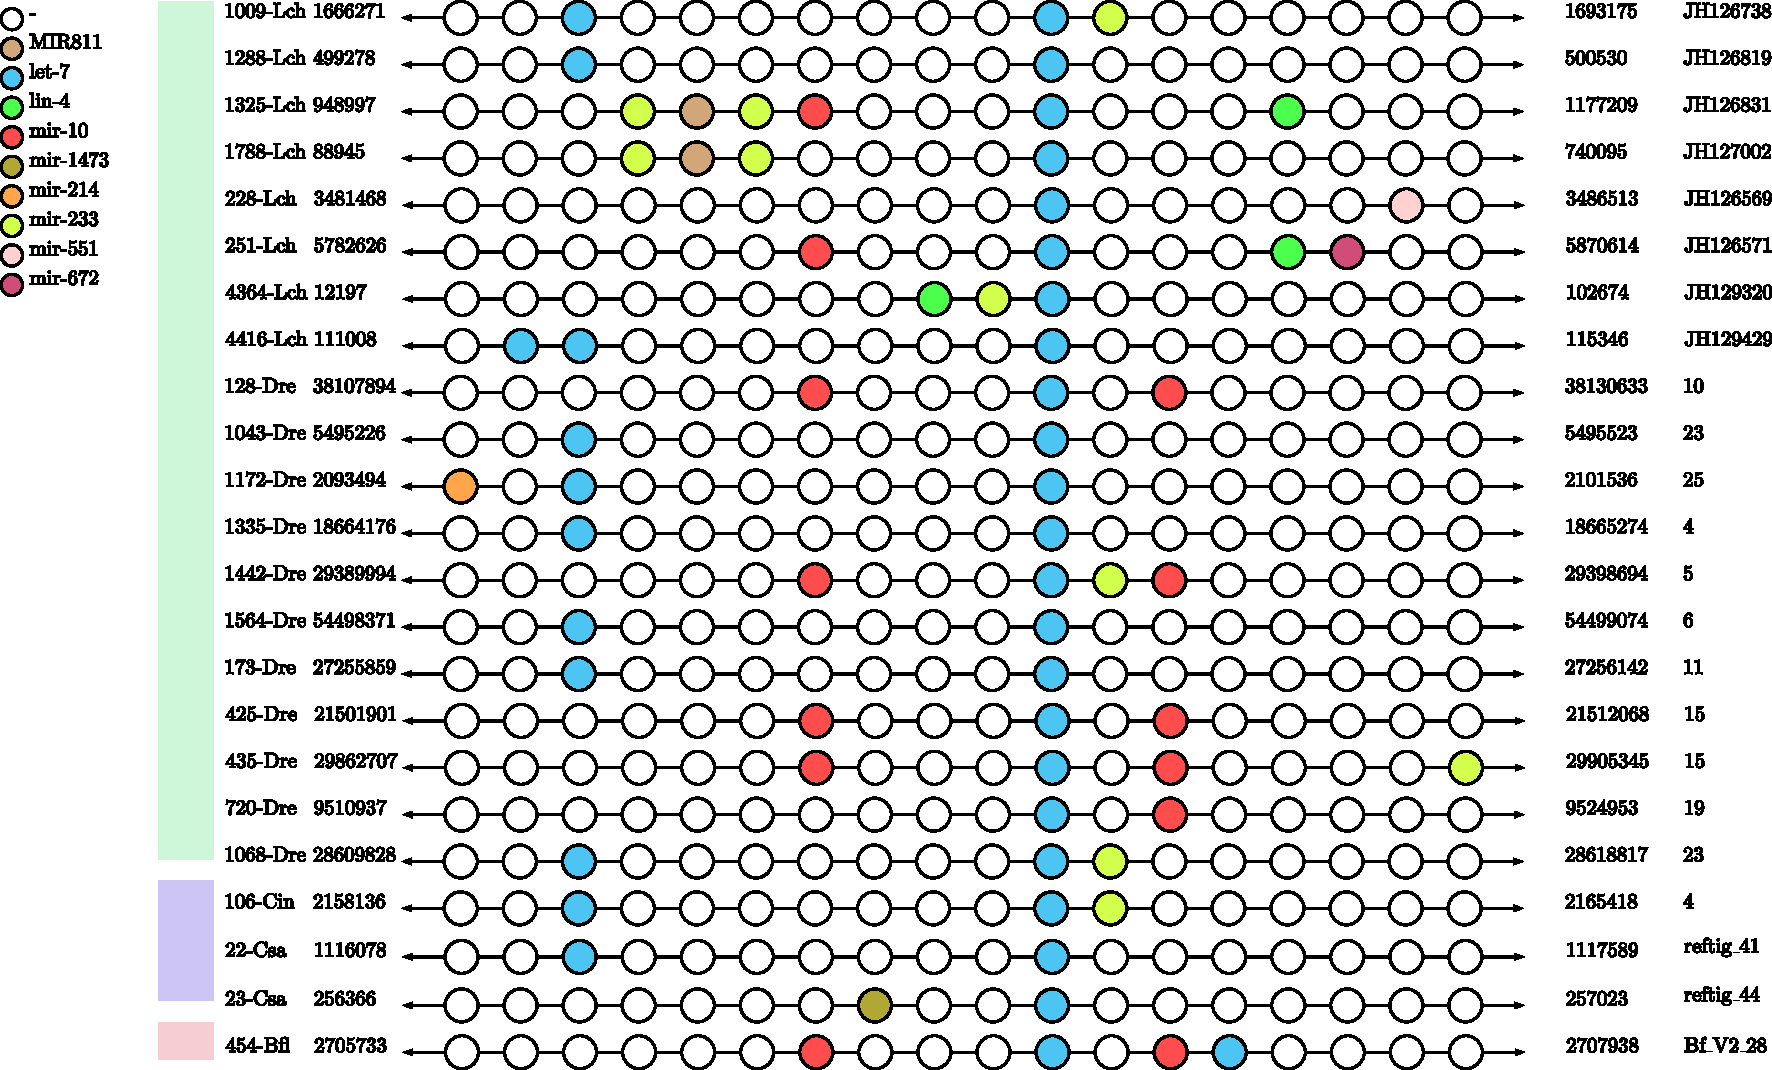
\includegraphics[height=9 cm]{./Images/Cluster_images/let-7_101_128}
        \caption{let-7}
    \end{subfigure}
    \\
    \begin{subfigure}[t]{0.45\textwidth}
        \centering
        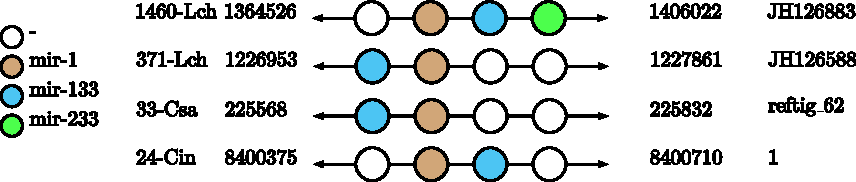
\includegraphics[height=1.2 cm]{./Images/Cluster_images/mir-1_119_33}
        \caption{mir-1/mir-133}
     \end{subfigure}
        ~
     \\
    \begin{subfigure}[t]{0.45\textwidth}
        \centering
        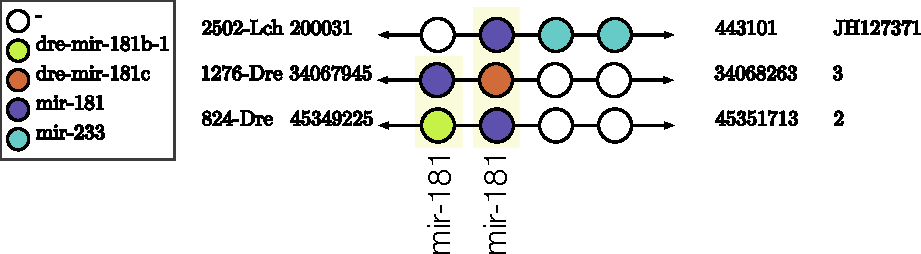
\includegraphics[height=1.2 
cm]{./Images/Cluster_images/mir-181_105_2502}
        \caption{mir-181}
       \end{subfigure}
        ~
         \begin{subfigure}[t]{0.45\textwidth}
        \centering
        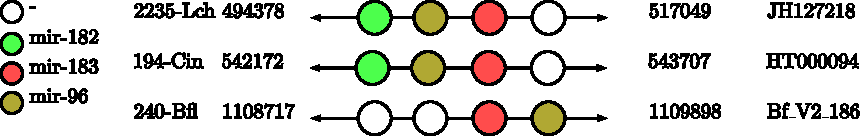
\includegraphics[height=1.2 cm]{./Images/Cluster_images/mir-183_132_240}
        \caption{mir-183}
    \end{subfigure}
    \\
    \begin{subfigure}[t]{0.45\textwidth}
        \centering
        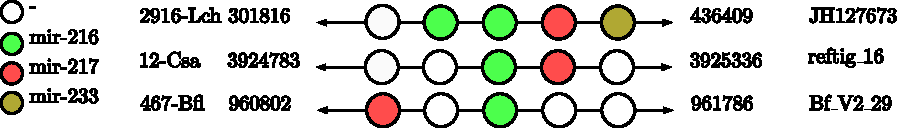
\includegraphics[height=1.2 cm]{./Images/Cluster_images/mir-216_126_467}
        \caption{mir-216/mir-217}
       \end{subfigure}
     \\
    \begin{subfigure}[t]{0.45\textwidth}
        \centering
        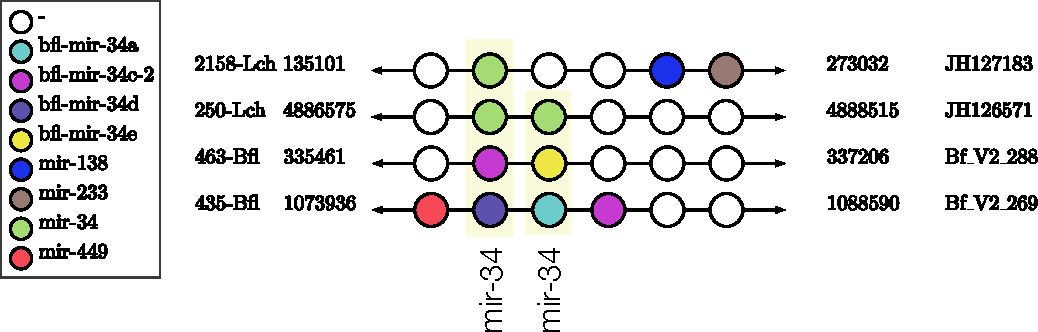
\includegraphics[height=1.2 cm]{./Images/Cluster_images/mir-34_11A_435}
        \caption{mir-34}
       \end{subfigure}
        ~
         \begin{subfigure}[t]{0.45\textwidth}
        \centering
        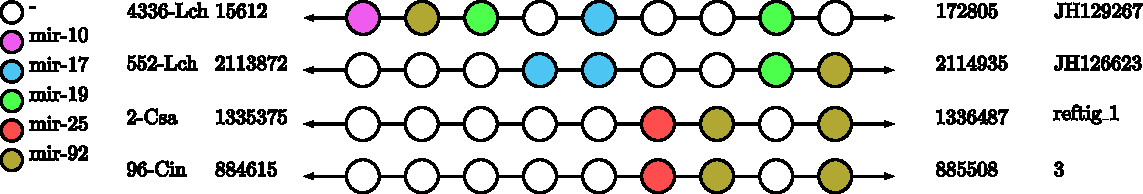
\includegraphics[height=1.2 cm]{./Images/Cluster_images/mir-92_281_4336}
        \caption{mir-92}
    \end{subfigure}
    \\
    \begin{subfigure}[t]{1\textwidth}
        \centering
        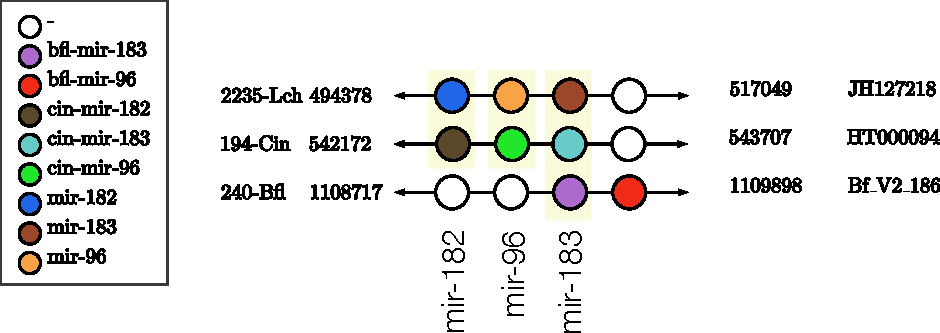
\includegraphics[height=1.2 cm]{./Images/Cluster_images/mir-96_138_240}
        \caption{mir-96}
    \end{subfigure}
    \caption{Multiple alignments of miRNA's clusters. \textbf{Prot}: 
Protostomata, \textbf{Brfl}: \textit{B. floridae}, 
\textbf{Oidi}: \textit{O. dioica}, \textbf{Dvex}: \textit{D. vexillum}, 
\textbf{Ciin}: \textit{C. intestinalis}, \textbf{Cisa}: \textit{C. savignyi}, 
\textbf{Ciro}: \textit{C. robusta}, \textbf{Sath}: \textit{S. thompsoni}, 
\textbf{Mata}: \textit{M. oculata}, \textbf{Mlta}: \textit{M. occulta}, 
\textbf{Mlis}: \textit{M. occidentalis}, \textbf{Bosc}: \textit{B. schlosseri}, 
\textbf{Haro}: \textit{H. roretzi}, \textbf{Pema}: \textit{P. marinus}, 
\textbf{Dare}: \textit{D. rerio}, \textbf{Lach}: \textit{L. chalumnae}, 
\textbf{Xetr}: \textit{X. tropicalis} and \textbf{Anca}: \textit{A. 
carolinensis}.}
\end{figure}

\subsubsection{Yanetal2014.pdf}

\cite{Yang2014}
\textit{mir181 is an ancient microRNA (miRNA) gene family that originated in urochordata. Although their functions were subjected to extensive studies in recent years, their evolutionary process remains largely unknown. Here we systematically investigated the homologous genes of the mir-181 family by a sequence similarity search. Representative sequences of the mir-181 gene family were used to reconstruct their evolutionary history. Our results indicated that this family could have derived from multiple duplications, which include two rounds of whole genome duplications and one round of segmental replication. Functional annotation of the target genes of the mir-181 family suggested that this family could participate in some important biological processes including transcriptional and translational regulation, signaling transduction etc. This analysis presented a complex evolutionary dynamics for the origination of a miRNA gene family.}

\subsubsection{Wangetal2017.pdf}
cite{Wang2017}
\textit{Background: miRNAs play essential roles in the modulation of cellular functions via degradation and/or translation
attenuation of target mRNAs. They have been surveyed in a single ascidian genus, Ciona. Recently, an annotated
draft genome sequence for a distantly related ascidian, Halocynthia roretzi, has become available, but miRNAs in
H. roretzi have not been previously studied.
Results: We report the prediction of 319 candidate H. roretzi miRNAs, obtained through three complementary
methods. Experimental validation suggests that more than half of these candidate miRNAs are expressed during
embryogenesis. The majority of predicted H. roretzi miRNAs appear specific to ascidians or tunicates, and only 32
candidates, belonging to 25 families, are widely conserved across metazoans.
Conclusion: Our study presents a comprehensive identification of candidate H. roretzi miRNAs. This resource
will facilitate the study of the mechanisms for miRNA-controlled gene regulatory networks during ascidian
development. Further, our analysis suggests that the majority of Halocynthia miRNAs are specific to ascidian
or tunicates, with only a small number of widely conserved miRNAs. This result is consistent with the general
notion that animal miRNAs are less conserved between taxa than plant ones.}

\subsubsection{deSouzaGomezetal2012.pdf}
\cite{DeSouzaGomes2013}
\textit{MicroRNAs (miRNAs) are small noncoding RNA molecules which are processed into {\~{}}20-24 nt molecules that can regulate the gene expression post-transcriptionally. MiRNA gene clusters have been identified in a range of species, where in miRNAs are often processed from polycistronic transcripts. In this study, a computational approach is used to investigate the extent of evolutionary conservation of the miR-71/2 cluster in animals, and to identify novel miRNAs in the miRNA cluster miR-71/2. The miR-71/2 cluster, consisting of copies of the miR-71 and miR-2 (including miR-13) families, was found to be Protostome-specific. Although, this cluster is highly conserved across the Protostomia, the miR-2 family is completely absent from the Deuterostomia species, while miR-71 is absent from the Vertebrata and Urochordata. The evolutionary conservation and clustering propensity of the miR-71/2 family across the Protostomes could indicate the common functional roles across the member species of the Protostomia.},

\subsubsection{Stadler2007.PDF}
\cite{Will2007}
\textit{The RFAM database defines families of ncRNAs by means of sequence similarities that are sufficient to establish homology. In some cases, such as microRNAs and box H/ACA snoRNAs, functional commonalities define classes of RNAs that are characterized by structural similarities, and typically consist of multiple RNA families. Recent advances in high-throughput transcriptomics and comparative genomics have produced very large sets of putative noncoding RNAs and regulatory RNA signals. For many of them, evidence for stabilizing selection acting on their secondary structures has been derived, and at least approximate models of their structures have been computed. The overwhelming majority of these hypothetical RNAs cannot be assigned to established families or classes. We present here a structure-based clustering approach that is capable of extracting putative RNA classes from genome-wide surveys for structured RNAs. The LocARNA (local alignment of RNA) tool implements a novel variant of the Sankoff algorithm that is sufficiently fast to deal with several thousand candidate sequences. The method is also robust against false positive predictions, i.e., a contamination of the input data with unstructured or nonconserved sequences. We have successfully tested the LocARNA-based clustering approach on the sequences of the RFAM-seed alignments. Furthermore, we have applied it to a previously published set of 3,332 predicted structured elements in the Ciona intestinalis genome (Missal K, Rose D, Stadler PF (2005) Noncoding RNAs in Ciona intestinalis. Bioinformatics 21 (Supplement 2): i77-i78). In addition to recovering, e.g., tRNAs as a structure-based class, the method identifies several RNA families, including microRNA and snoRNA candidates, and suggests several novel classes of ncRNAs for which to date no representative has been experimentally characterized.}

\subsection{miRNA in an perspective evolution}

\subsubsection{Introduction}

\subsubsection{Pignatelli2016.pdf}
\cite{Pignatelli2016}
\textit{Annotation of orthologous and paralogous genes is necessary for many aspects of evolutionary analysis. Methods to infer these homology relationships have traditionally focused on protein-coding genes and evolutionary models used by these methods normally assume the positions in the protein evolve independently. However, as our appreciation for the roles of non-coding RNA genes has increased, consistently annotated sets of orthologous and paralogous ncRNA genes are increasingly needed. At the same time, methods such as PHASE or RAxML have implemented substitution models that consider pairs of sites to enable proper modelling of the loops and other features of RNA secondary structure. Here, we present a comprehensive analysis pipeline for the automatic detection of orthologues and paralogues for ncRNA genes. We focus on gene families represented in Rfam and for which a specific covariance model is provided. For each family ncRNA genes found in all Ensembl species are aligned using Infernal, and several trees are built using different substitution models. In parallel, a genomic alignment that includes the ncRNA genes and their flanking sequence regions is built with PRANK. This alignment is used to create two additional phylogenetic trees using the neighbour-joining (NJ) and maximum-likelihood (ML) methods. The trees arising from both the ncRNA and genomic alignments are merged using TreeBeST, which reconciles them with the species tree in order to identify speciation and duplication events. The final tree is used to infer the orthologues and paralogues following Fitch's definition. We also determine gene gain and loss events for each family using CAFE. All data are accessible through the Ensembl Comparative Genomics ('Compara') API, on our FTP site and are fully integrated in the Ensembl genome browser, where they can be accessed in a user-friendly manner.Database URL: http://www.ensembl.org.}
\subsubsection{Dai2009.pdf}

\cite{Dai2009}
\textit{Cephalochordates, urochordates, and vertebrates comprise the three extant groups of chordates. Although higher morphological and developmental similarity exists between cephalochordates and vertebrates, molecular phylogeny studies have instead suggested that the morphologically simplified urochordates are the closest relatives to vertebrates. MicroRNAs (miRNAs) are regarded as the major factors driving the increase of morphological complexity in early vertebrate evolution, and are extensively characterized in vertebrates and in a few species of urochordates. However, the comprehensive set of miRNAs in the basal chordates, namely the cephalochordates, remains undetermined. Through extensive sequencing of a small RNA library and genomic homology searches, we characterized 100 miRNAs from the cephalochordate amphioxus, Branchiostoma japonicum, and B. floridae. Analysis of the evolutionary history of the cephalochordate miRNAs showed that cephalochordates possess 54 miRNA families homologous to those of vertebrates, which is threefold higher than those shared between urochordates and vertebrates. The miRNA contents demonstrated a clear correlation between the extent of miRNA overlapping and morphological similarity among the three chordate groups, providing a strong evidence of miRNAs being the major genetic factors driving morphological complexity in early chordate evolution.}
\subsubsection{Candini2012.pdf}
\cite{Candiani2012}
\textit{MicroRNAs (miRNAs) are small non-coding RNAs that negatively regulate gene expression and thus control diverse biological processes. The high interest in miRNAs as an important mediator of post-transcriptional gene regulation has led to the discovery of miRNAs in several organisms. The present article outlines and discusses the current status of miRNAs information on the basal chordate amphioxus and the evolution of miRNAs in metazoans.}

\subsubsection{Stadler2006.pdf}
\cite{Hertel2006}
\textit{UNLABELLED: Recently, genome-wide surveys for non-coding RNAs have provided evidence for tens of thousands of previously undescribed evolutionary conserved RNAs with distinctive secondary structures. The annotation of these putative ncRNAs, however, remains a difficult problem. Here we describe an SVM-based approach that, in conjunction with a non-stringent filter for consensus secondary structures, is capable of efficiently recognizing microRNA precursors in multiple sequence alignments. The software was applied to recent genome-wide RNAz surveys of mammals, urochordates, and nematodes. AVAILABILITY: The program RNAmicro is available as source code and can be downloaded from http://www.bioinf.uni-leipzig/Software/RNAmicro.}

\subsubsection{SamGriffit2007.pdf}
\cite{Griffiths-Jones2011}
\textit{MicroRNAs (miRNAs) modulate transcript stability and translation. Functional mature miRNAs are processed from one or both arms of the hairpin precursor. The miR-100/10 family has undergone three independent evolutionary events that have switched the arm from which the functional miRNA is processed. The dominant miR-10 sequences in the insects Drosophila melanogaster and Tribolium castaneum are processed from opposite arms. However, the duplex produced by Dicer cleavage has an identical sequence in fly and beetle. Expression of the Tribolium miR-10 sequence in Drosophila S2 cells recapitulates the native beetle pattern. Thus, arm usage is encoded in the primary miRNA sequence, but outside the mature miRNA duplex. We show that the predicted messenger RNA targets and inferred function of sequences from opposite arms differ significantly. Arm switching is likely to be general, and provides a fundamental mechanism to evolve the function of a miRNA locus and target gene network.},
author = {Griffiths-Jones, Sam and Hui, Jerome H L and Marco, Antonio and Ronshaugen, Matthew}

\subsubsection{Hertel2015.pdf}
\cite{Hertel2015}
\textit{MicroRNAs are important regulatory small RNAs in many eukaryotes. Due to their small size and simple structure, they are readily innovated de novo. Throughout the evolution of animals, the emergence of novel microRNA families traces key morphological innovations. Here, we use a computational approach based on homology search and parsimony-based presence/absence analysis to draw a comprehensive picture of microRNA evolution in 159 animal species. We confirm previous observations regarding bursts of innovations accompanying the three rounds of genome duplications in vertebrate evolution and in the early evolution of placental mammals. With a much better resolution for the invertebrate lineage compared to large-scale studies, we observe additional bursts of innovation, e.g., in Rhabditoidea. More importantly, we see clear evidence that loss of microRNA families is not an uncommon phenomenon. The Enoplea may serve as a second dramatic example beyond the tunicates. The large-scale analysis presented here also highlights several generic technical issues in the analysis of very large gene families that will require further research.}

\subsubsection{Yanetal2014.pdf}


\cite{Yang2014}
\textit{Mir-181 is an ancient microRNA (miRNA) gene family that originated in urochordata. Although their functions were subjected to extensive studies in recent years, their evolutionary process remains largely unknown. Here we systematically investigated the homologous genes of the mir-181 family by a sequence similarity search. Representative sequences of the mir-181 gene family were used to reconstruct their evolutionary history. Our results indicated that this family could have derived from multiple duplications, which include two rounds of whole genome duplications and one round of segmental replication. Functional annotation of the target genes of the mir-181 family suggested that this family could participate in some important biological processes including transcriptional and translational regulation, signaling transduction etc. This analysis presented a complex evolutionary dynamics for the origination of a miRNA gene family. {\textcopyright} 2014 Elsevier Ltd.}


\subsection{To complete the tree of loss and gain of families}

\begin{figure}[ht!]
\centering 
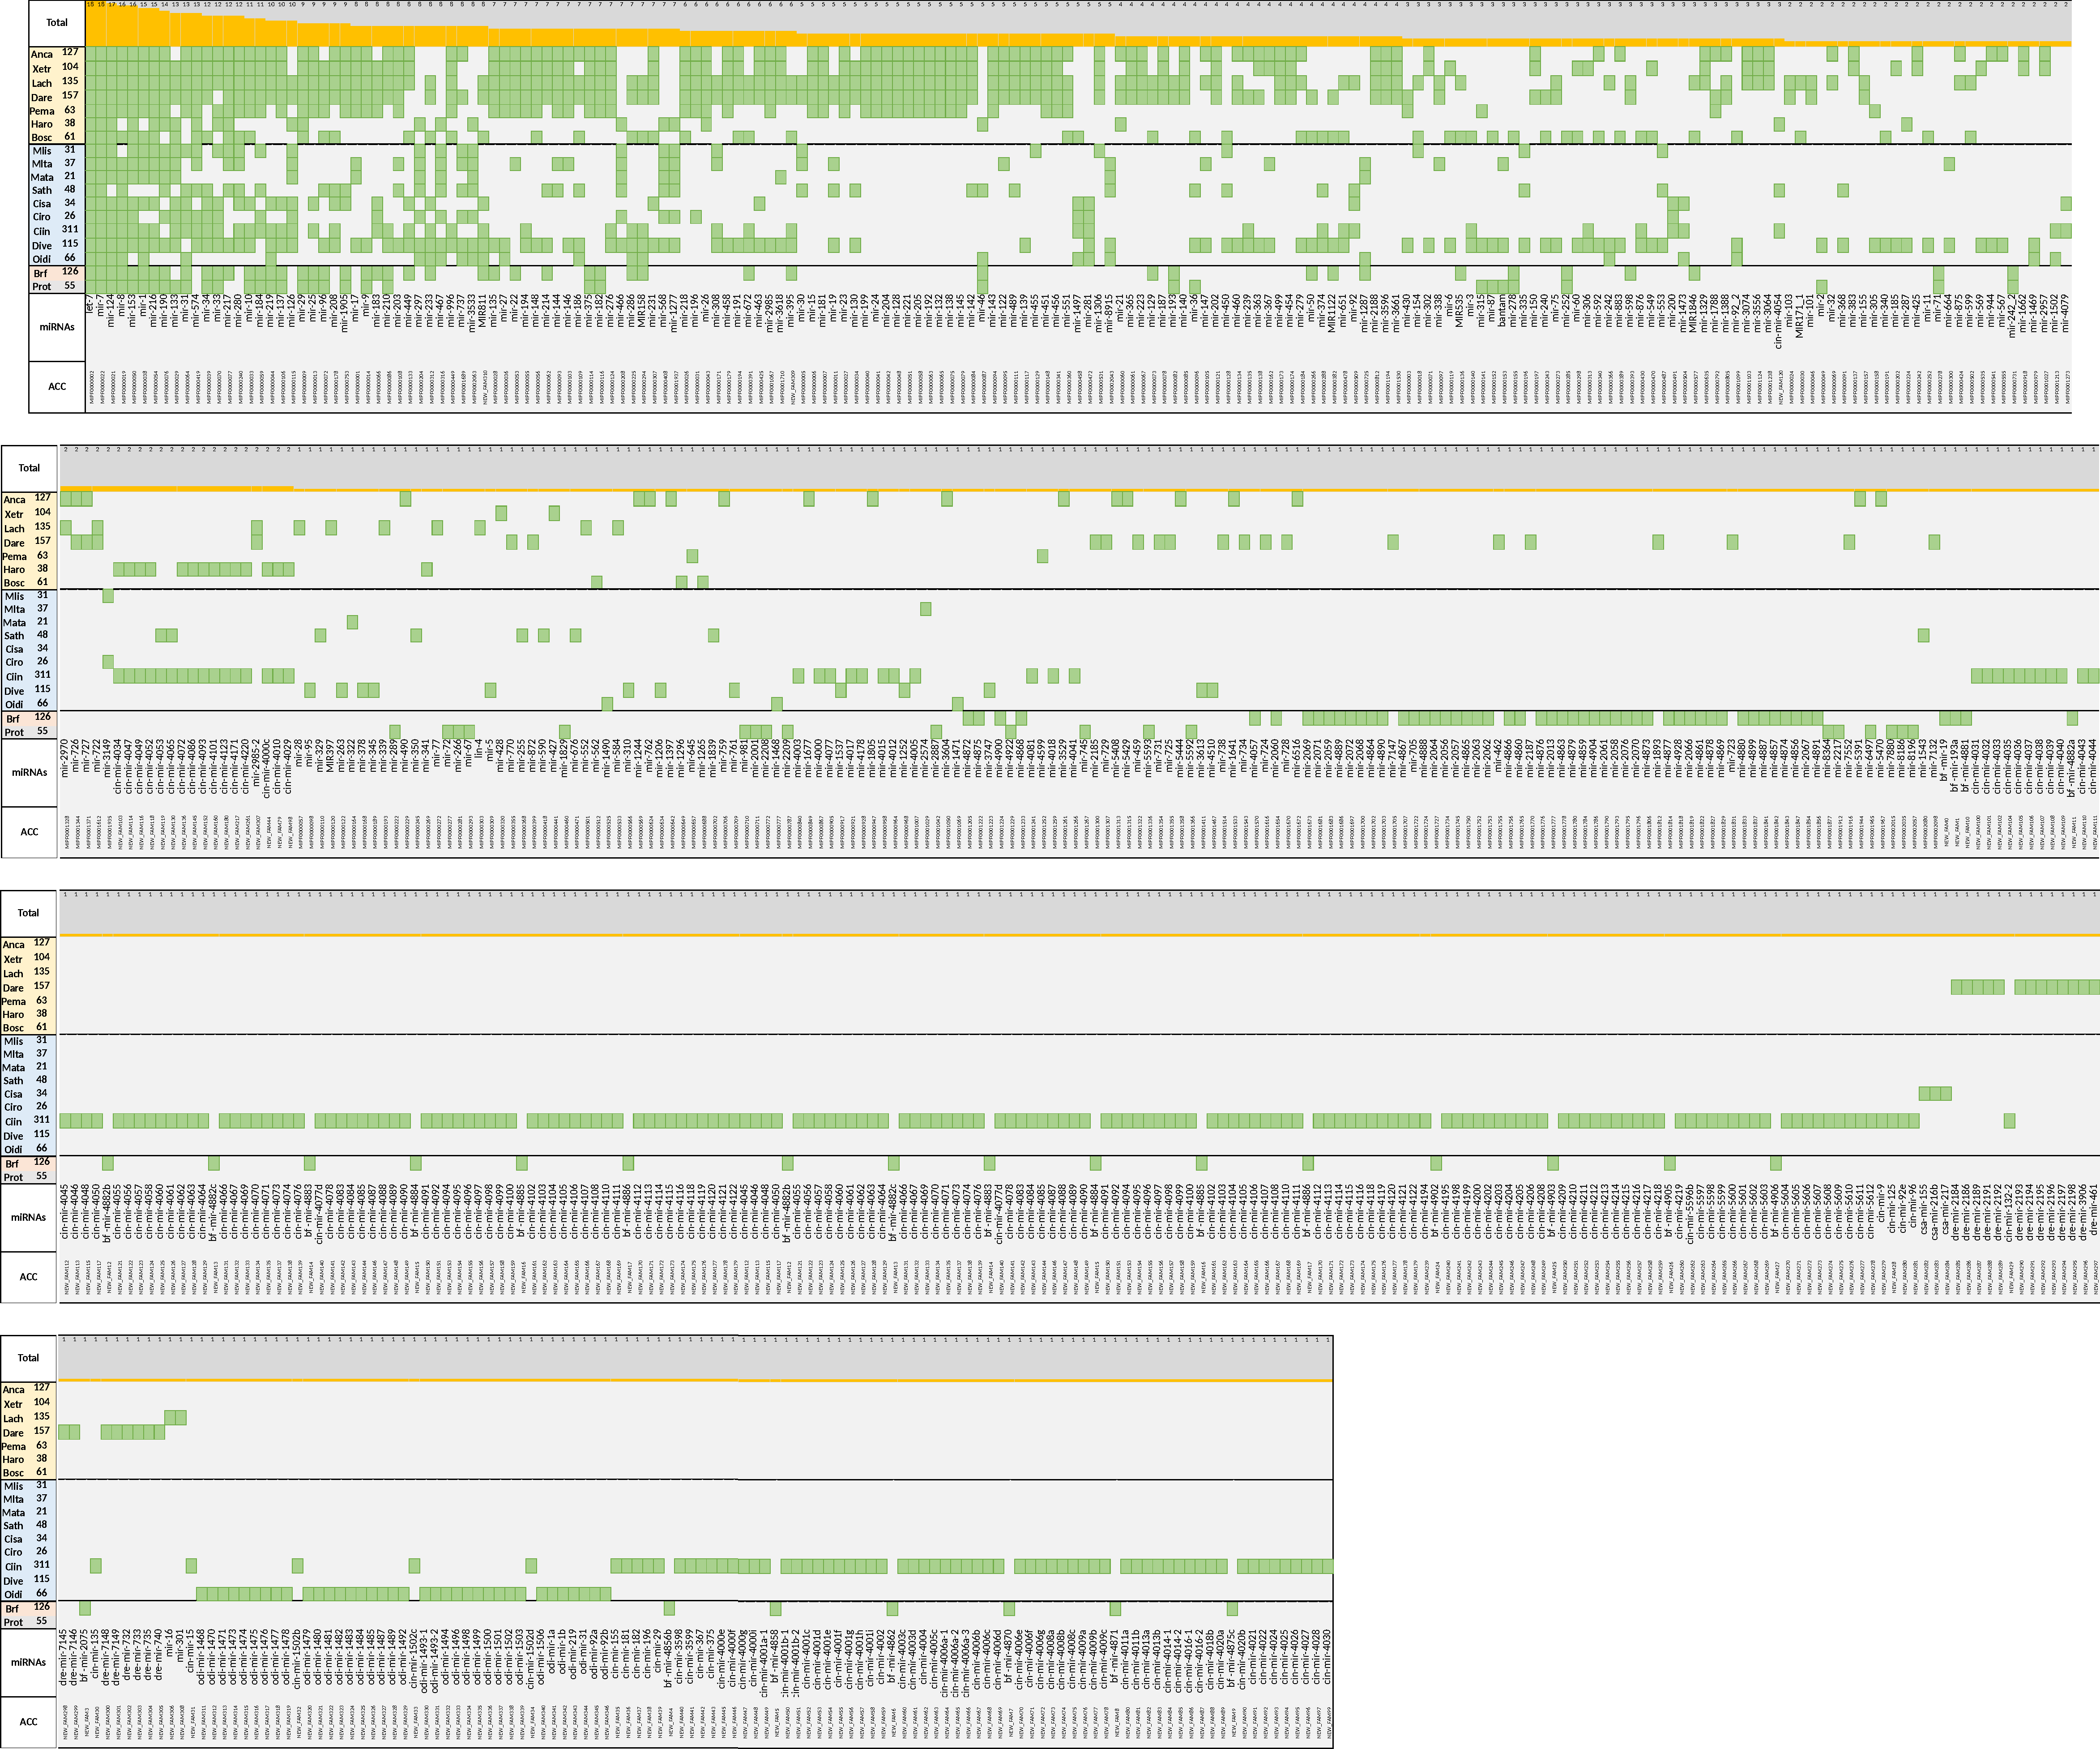
\includegraphics[width=\textwidth]{./Images/miRNA_matrix}
\caption{Absence/Presence Matrix of miRNAs families along Bilaterian species. 
\textbf{Prot}: Protostomata, \textbf{Brfl}: \textit{B. floridae}, 
\textbf{Oidi}: \textit{O. dioica}, \textbf{Dvex}: \textit{D. vexillum}, 
\textbf{Ciin}: \textit{C. intestinalis}, \textbf{Cisa}: \textit{C. savignyi}, 
\textbf{Ciro}: \textit{C. robusta}, \textbf{Sath}: \textit{S. thompsoni}, 
\textbf{Mata}: \textit{M. oculata}, \textbf{Mlta}: \textit{M. occulta}, 
\textbf{Mlis}: \textit{M. occidentalis}, \textbf{Bosc}: \textit{B. schlosseri}, 
\textbf{Haro}: \textit{H. roretzi}, \textbf{Pema}: \textit{P. marinus}, 
\textbf{Dare}: \textit{D. rerio}, \textbf{Lach}: \textit{L. chalumnae}, 
\textbf{Xetr}: \textit{X. tropicalis} and \textbf{Anca}: \textit{A. 
carolinensis}. }
\label{fig:matrimirnas}
\end{figure}

Our miRNA families updated with the new two annotated miRNAs Salpa and 
Halocyntia

\begin{figure}[ht!]
\centering
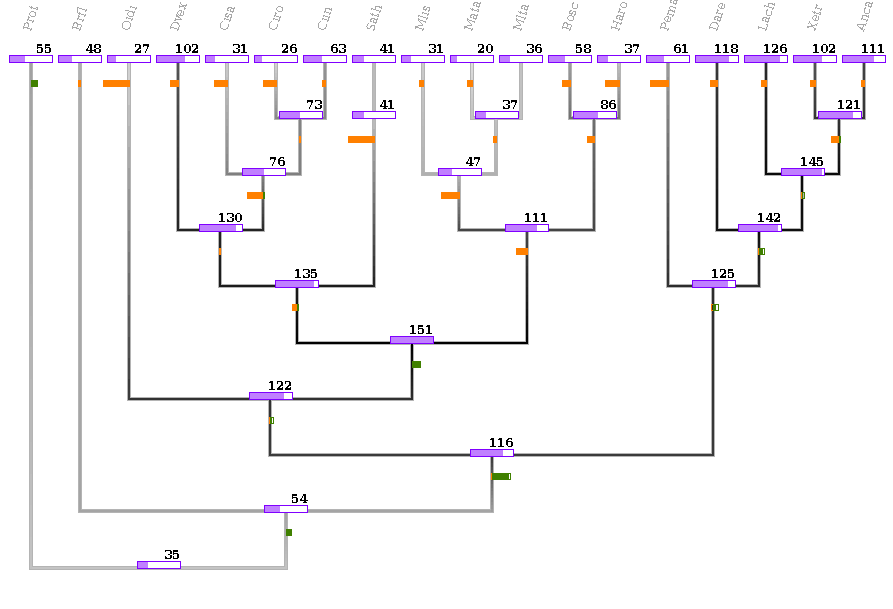
\includegraphics[width=\textwidth]{./Images/last_tree.png}
\caption{Dollo parsymony of miRNAs families distribution in some 
chordates genomes}.
\label{fig:dollotree}
\end{figure}

\cite{velandia:2016} \textit{A comparative analysis of miRNAs families in 
tunicates is summarized in Fig. 5 c and d. We find several patterns of 
recognizable trends as we analyze the conservation, loss and gain of miRNA 
families in tunicates compared to selected bilaterians. For instance, based in 
our analysis of conserved miRNA families across the bilaterians, we estimate 
that ancestor of the Bilateria likely contained approximately 33 miRNA families. 
In contrast, the ancestor of the Chordata presumably contained members of 37 
miRNA families. In the cephalochordate B. floridae, we find the occurrence of a 
unique repertoire of 82 miRNA families that evolved as a consequence of many 
gains (+50), but also some losses (−5) [8]. In the ancestor of Olfactores we 
presume the presence of 72 miRNA families, of which tunicates did not show 
losses, with the notable exception of O. dioica that has undergone substantial 
losses (−60). Within the ascidians, only B. schlosseri and C. savignyi show 
dramatic losses of miRNA families, −32 and −17 respectively. D. vexillum has 
lost 8 miRNA families. D. vexillum shows 16 families that are absent in other 
tunicates i.e. mir-430, mir-9, mir-130, mir-190, mir-139, mir-460, mir-315, 
mir-305, mir-458, mir-185, mir-233, mir-569, mir-944, mir-567, mir-2985 and 
mir-4068 (Fig. 5d). Comparisons of the miRNAs repertoires between the colonial 
tunicates (D. vexillum and B. schlosseri) on the one hand, and solitary 
tunicates (O. dioica, C. intestinalis and C. savignyi) on the other hand, show 
10 microRNA families, i.e. mir-133, mir-186, mir-6, mir-279, mir-340, mir-11, 
mir-60, mir-592, mir-883 and mir-549 that are specific to colonial tunicates, 
while only 2 families, i.e. mir-31 and mir-1473, are specific to olitary 
tunicates. It is worthwhile exploring how colonial specific miRNAs may have been 
co-opted in ascidians to function in somatic stem cell function, regeneration, 
budding, or other asexual developmental processes, as miRNAs are know to be 
important players in stem cell function, and developmental processes of 
differentiation in vertebrates}



\subsubsection{Jueetal2016.pdf}
\cite{Jue2016,}
\textit{A preliminary genome sequence has been assembled for the Southern Ocean salp, Salpa thompsoni (Urochordata, Thaliacea). Despite the ecological importance of this species in Antarctic pelagic food webs and its potential role as an indicator of changing Southern Ocean ecosystems in response to climate change, no genomic resources are available for S. thompsoni or any closely-related urochordate species. Using a multiple-platform, multiple-individual approach, we have produced a 318,767,936 bp genome sequence, covering more than 50{\%} of the estimated 602 MB (±173 MB) genome size for S. thompsoni Using a non-redundant set of predicted proteins, more than 50{\%} (16,823) of sequences showed significant homology to known proteins and {\~{}}38{\%} (12,151) of the total protein predictions were associated with Gene Ontology functional information. We have generated 109,958 SNP variant and 9,782 indel predictions for this species, serving as a resource for future phylogenomic and population genetic studies. Comparing the salp genome to available assemblies for four other urochordates, Botryllus schlosseri, Ciona intestinalis, Ciona savignyi and Oikopleura dioica, we found that S. thompsoni shares the previously-estimated rapid rates of evolution for these species. High mutation rates are thus independent of genome size, suggesting that rates of evolution {\textgreater}1.5 times that observed for vertebrates are a broad taxonomic characteristic of urochordates. Tests for positive selection implemented in PAML revealed a small number of genes with sites undergoing rapid evolution, including genes involved in ribosome biogenesis and metabolic and immune process that may be reflective of both adaptation to polar, planktonic environments as well as the complex life history of the salps. Finally, we performed an initial survey of small RNAs, revealing the presence of known, conserved miRNAs, as well as novel miRNA genes; unique piRNAs; and mature miRNA signatures for varying developmental stages. Collectively, these resources provide a genomic foundation supporting S. thompsoni as a model species for further examination of the exceptional rates and patterns of genomic evolution shown by urochordates. Additionally, genomic data will allow for the development of molecular indicators of key life history events and processes and afford new understandings and predictions of impacts of climate change on this key species of Antarctic pelagic ecosystems.}


\subsubsection{Wangetal2017.pdf}
\cite{Wang2017}
\textit{Background: miRNAs play essential roles in the modulation of cellular functions via degradation and/or translation
attenuation of target mRNAs. They have been surveyed in a single ascidian genus, Ciona. Recently, an annotated
draft genome sequence for a distantly related ascidian, Halocynthia roretzi, has become available, but miRNAs in
H. roretzi have not been previously studied.
Results: We report the prediction of 319 candidate H. roretzi miRNAs, obtained through three complementary
methods. Experimental validation suggests that more than half of these candidate miRNAs are expressed during
embryogenesis. The majority of predicted H. roretzi miRNAs appear specific to ascidians or tunicates, and only 32
candidates, belonging to 25 families, are widely conserved across metazoans.
Conclusion: Our study presents a comprehensive identification of candidate H. roretzi miRNAs. This resource
will facilitate the study of the mechanisms for miRNA-controlled gene regulatory networks during ascidian
development. Further, our analysis suggests that the majority of Halocynthia miRNAs are specific to ascidian
or tunicates, with only a small number of widely conserved miRNAs. This result is consistent with the general
notion that animal miRNAs are less conserved between taxa than plant ones.}

\section{miRNAs and its rol in development}
\label{sec:3}

\subsection{miRNAs discovery and development}

\subsubsection{Bartel2004.pdf}

\cite{Bartel2004}
\textit{MicroRNAs (miRNAs) are endogenous ???22 nt RNAs that can play important regulatory roles in animals and plants by targeting mRNAs for cleavage or translational repression. Although they escaped notice until relatively recently, miRNAs comprise one of the more abundant classes of gene regulatory molecules in multicellular organisms and likely influence the output of many protein-coding genes.}
\subsubsection{Lee1993.pdf}

\cite{Lee1993}
\textit{diverse postembryonic developmental events in C.
elegans. /in-4 acts by negatively regulating the level of
LIN-14 protein, creating a temporal decrease in LIN-14
protein starting in the first larval stage (Ll). We have
cloned the C. elegans lin-4 locus by chromosomal
walking and transformation rescue. We used the C.
elegans clone to isolate the gene from three other
Caenorhabditis species; all four Caenorhabditis clones
functionally rescue the h-4 null allele of C. elegans.
Comparison of the /in-4 genomic sequence from these
four species and site-directed mutagenesis of potential
open reading frames indicated that /in-d does not
encode a protein. Two small /in-4 transcripts of approximately
22 and 61 nt were identified in C. elegans and
found to contain sequences complementary to a repeated
sequence element in the 3'untranslated region
(UTR) of lin-74 mRNA, suggesting that /in-4 regulates
h-74 tr}


\subsection{miRNAs perspective evolution in development}

\subsubsection{holland2014.pdf}
\cite{Holland2015} \textit{
Morphological comparisons among extant animals have long been used to infer 
their long-extinct ancestors for which the fossil record is poor or 
non-existent. For evolution of the vertebrates, the comparison has typically 
involved amphioxus and vertebrates. Both groups are evolving relatively slowly, 
and their genomes share a high level of synteny. Both vertebrates and amphioxus 
have regulative development in which cell fates become fixed only gradually 
during embryogenesis. Thus, their development fits a modified hourglass model in 
which constraints are greatest at the phylotypic stage (i.e., the late 
neurula/early larva), but are somewhat greater on earlier development than on 
later development. In contrast, the third group of chordates, the tunicates, 
which are sister group to vertebrates, are evolving rapidly. Constraints on 
evolution of tunicate genomes are relaxed, and they have discarded key 
developmental genes and organized much of their coding sequences into operons, 
which are transcribed as a single mRNA that undergoes trans-splicing. This 
contrasts with vertebrates and amphioxus, whose genomes are not organized into 
operons. Concomitantly, tunicates have switched to determinant development with 
very early fixation of cell fates. Thus, tunicate development more closely fits 
a progressive divergence model (shaped more like a wine glass than an hourglass) 
in which the constraints on the zygote and very early development are greatest. 
This model can help explain why tunicate body plans are so very diverse. The 
relaxed constraints on development after early cleavage stages are correlated 
with relaxed constraints on genome evolution. The question remains: which came 
first?}
\subsubsection{Sun2013.pdf}

\cite{Sun2013}
\textit{MicroRNAs (miRNAs) are {\~{}}22 nt RNAs that coordinate vast regulatory 
networks in animals and thereby influence myriad processes. This Review examines 
evidence that miRNAs have continuous roles in adults in ways that are separable 
from developmental control. Adult-specific activities for miRNAs have been 
described in various stem cell populations, in the context of neural function 
and cardiovascular biology, in metabolism and ageing, and during cancer. In 
addition to reviewing recent results, we also discuss methods for studying miRNA 
activities specifically in adults and evaluate their relative strengths and 
weaknesses. A fuller understanding of continuous functions of miRNAs in adults 
has bearing on efforts and opportunities to manipulate miRNAs for therapeutic 
purposes.}
\subsubsection{Kloosterman2006.pdf}

\cite{Kloosterman2006}
\textit{MicroRNAs (miRNAs) control gene expression by translational inhibition 
and destabilization of mRNAs. While hundreds of miRNAs have been found, only??a 
few have been studied in detail. miRNAs have been implicated in tissue 
morphogenesis, cellular processes like apoptosis, and major signaling pathways. 
Emerging evidence suggests a direct link between miRNAs and disease, and miRNA 
expression signatures are associated with various types of cancer. In addition, 
the gain and loss of miRNA target sites appears to be causal to some genetic 
disorders. Here, we discuss the current literature on the role of miRNAs in 
animal development and disease. ?? 2006 Elsevier Inc. All rights reserved.}

\subsubsection{Iyengar2014.pdf}

\cite{Iyengar2014}
\textit{The human brain is one of the most complex biological systems, and the 
cognitive abilities have greatly expanded compared to invertebrates without much 
expansion in the number of protein coding genes. This suggests that gene 
regulation plays a very important role in the development and function of 
nervous system, by acting at multiple levels such as transcription and 
translation. In this article we discuss the regulatory roles of three classes of 
non-protein coding RNAs (ncRNAs)-microRNAs (miRNAs), piwi-interacting RNA 
(piRNAs) and long-non-coding RNA (lncRNA), in the process of neurogenesis and 
nervous function including control of synaptic plasticity and potential roles in 
neurodegenerative diseases. miRNAs are involved in diverse processes including 
neurogenesis where they channelize the cellular physiology toward neuronal 
differentiation. miRNAs can also indirectly influence neurogenesis by regulating 
the proliferation and self renewal of neural stem cells and are dysregulated in 
several neurodegenerative diseases. miRNAs are also known to regulate synaptic 
plasticity and are usually found to be co-expressed with their targets. The 
dynamics of gene regulation is thus dependent on the local architecture of the 
gene regulatory network (GRN) around the miRNA and its targets. piRNAs had been 
classically known to regulate transposons in the germ cells. However, piRNAs 
have been, recently, found to be expressed in the brain and possibly function by 
imparting epigenetic changes by DNA methylation. piRNAs are known to be 
maternally inherited and we assume that they may play a role in early 
development. We also explore the possible function of piRNAs in regulating the 
expansion of transposons in the brain. Brain is known to express several lncRNA 
but functional roles in brain development are attributed to a few lncRNA while 
functions of most of the them remain unknown. We review the roles of some known 
lncRNA and explore the other possible functions of lncRNAs including their 
interaction with miRNAs.}

\subsection{Specific examples} 
\subsubsection{Chenetal2014.PDF}
\cite{Chen2014}
\textit{Notch-Delta signaling is a fundamental cell-cell communication mechanism 
that governs the differentiation of many cell types. Most existing mathematical 
models of Notch-Delta signaling are based on a feedback loop between Notch and 
Delta leading to lateral inhibition of neighboring cells. These models result in 
a checkerboard spatial pattern whereby adjacent cells express opposing levels of 
Notch and Delta, leading to alternate cell fates. However, a growing body of 
biological evidence suggests that Notch-Delta signaling produces other patterns 
that are not checkerboard, and therefore a new model is needed. Here, we present 
an expanded Notch-Delta model that builds upon previous models, adding a local 
Notch activity gradient, which affects long-range patterning, and the activity 
of a regulatory microRNA. This model is motivated by our experiments in the 
ascidian Ciona intestinalis showing that the peripheral sensory neurons, whose 
specification is in part regulated by the coordinate activity of Notch-Delta 
signaling and the microRNA miR-124, exhibit a sparse spatial pattern whereby 
consecutive neurons may be spaced over a dozen cells apart. We perform rigorous 
stability and bifurcation analyses, and demonstrate that our model is able to 
accurately explain and reproduce the neuronal pattern in Ciona. Using Monte 
Carlo simulations of our model along with miR-124 transgene over-expression 
assays, we demonstrate that the activity of miR-124 can be incorporated into the 
Notch decay rate parameter of our model. Finally, we motivate the general 
applicability of our model to Notch-Delta signaling in other animals by 
providing evidence that microRNAs regulate Notch-Delta signaling in analogous 
cell types in other organisms, and by discussing evidence in other organisms of 
sparse spatial patterns in tissues where Notch-Delta signaling is active.}

\subsubsection{Fuetal2008.pdf}

\cite{Fu2008}
\textit{Recent studies reveal correlation between microRNA (miRNA) innovation 
and increased developmental complexity. This is exemplified by dramatic 
expansion of the miRNA inventory in vertebrates, a lineage where genome 
duplication has played a significant evolutionary role. Urochordates, the 
closest extant group to the vertebrates, exhibit an opposite trend to genome and 
morphological simplification. We show that the urochordate, larvacean, 
Oikopleura dioica, possesses the requisite miRNA biogenic machinery. The miRNAs 
isolated by small RNA cloning were expressed throughout the short life cycle, a 
number of which were stocked as maternal determinants prior to rapid embryonic 
development. We identify sex-specific miRNAs that appeared as male/female gonad 
differentiation became apparent and were maintained throughout spermatogenesis. 
Whereas 80{\%} of mammalian miRNAs are hosted in introns of protein-coding 
genes, the majority of O. dioica miRNA loci were located in antisense 
orientations to such genes. Including sister group ascidians in analysis of the 
urochordate miRNA repertoire, we find that 11 highly conserved bilaterian miRNA 
families have been lost or derived to the point they are not recognizable in 
urochordates and a further 4 of these families are absent in larvaceans. 
Subsequent to this loss/derivation, at least 29 novel miRNA families have been 
acquired in larvaceans. This suggests a profound reorganization of the miRNA 
repertoire integral to evolution in the urochordate lineage.}

\subsubsection{Hendrixetal2010.pdf}
\cite{Hendrix2010}
\textit{MicroRNAs (miRs) have been broadly implicated in animal development and 
disease. We developed a novel computational strategy for the systematic, 
whole-genome identification of miRs from high throughput sequencing information. 
This method, miRTRAP, incorporates the mechanisms of miR biogenesis and includes 
additional criteria regarding the prevalence and quality of small RNAs arising 
from the antisense strand and neighboring loci. This program was applied to the 
simple chordate Ciona intestinalis and identified nearly 400 putative miR loci.}

\subsubsection{Kusakabeetal2013.pdf}
\cite{Kusakabe2013}
\textit{Muscle-specific miR-1/206 and miR-133 families have been suggested to 
play fundamental roles in skeletal and cardiac myogenesis in vertebrates. To 
gain insights into the relationships between the divergence of these miRs and 
muscular tissue types, we investigated the expression patterns of miR-1 and 
miR-133 in two ascidian Ciona species and compared their genomic structures with 
those of other chordates. We found that Ciona intestinalis and Ciona savignyi 
each possess a single copy of the miR-1/miR-133 cluster, which is only 350 
nucleotide long. During embryogenesis, Ciona miR-1 and miR-133 are generated as 
a single continuous primary transcript accumulated in the nuclei of the tail 
muscle cells, starting at the gastrula stage. In adults, mature miR-133 and 
miR-1 are differentially expressed in the heart and body wall muscle. Expression 
of the reporter gene linked to the 850-bp upstream region of the predicted 
transcription start site confirmed that this region drives the muscle-specific 
expression of the primary transcript of miR-1/miR-133. In many deuterostome 
lineages, including that of Ciona, the miR-1/133 cluster is located in the same 
intron of the mind bomb (mib) gene in reverse orientation. Our results suggest 
that the origin of genomic organization and muscle-specific regulation of 
miR-1/133 can be traced back to the ancestor of chordates. Duplication of this 
miR cluster might have led to the remarkable elaboration in the morphology and 
function of skeletal muscles in the vertebrate lineage. {\textcopyright} 2012 
Elsevier B.V. All rights reserved.}

\subsubsection{Pasquinellietal2000.pdf}

\cite{Pasquinelli2000}
\textit{Two small RNAs regulate the timing of Caenorhabditis elegans 
development. Transition from the first to the second larval stage fates requires 
the 22-nucleotide lin-4 RNA, and transition from late larval to adult cell fates 
requires the 21-nucleotide let-7 RNA. The lin-4 and let-7 RNA genes are not 
homologous to each other, but are each complementary to sequences in the 3' 
untranslated regions of a set of protein-coding target genes that are normally 
negatively regulated by the RNAs. Here we have detected let-7 RNAs of 
approximately 21 nucleotides in samples from a wide range of animal species, 
including vertebrate, ascidian, hemichordate, mollusc, annelid and arthropod, 
but not in RNAs from several cnidarian and poriferan species, Saccharomyces 
cerevisiae, Escherichia coli or Arabidopsis. We did not detect lin-4 RNA in 
these species. We found that let-7 temporal regulation is also conserved: let-7 
RNA expression is first detected at late larval stages in C. elegans and 
Drosophila, at 48 hours after fertilization in zebrafish, and in adult stages of 
annelids and molluscs. The let-7 regulatory RNA may control late temporal 
transitions during development across animal phylogeny.}

\subsubsection{Tangetal2013.pdf}
\textit{JoyceTang2013}
\textit{The formation of the sensory organs and cells that make up the 
peripheral nervous system (PNS) relies on the activity of transcription factors 
encoded by proneural genes (PNGs). Although PNGs have been identified in the 
nervous systems of both vertebrates and invertebrates, the complexity of their 
interactions has complicated efforts to understand their function in the context 
of their underlying regulatory networks. To gain insight into the regulatory 
network of PNG activity in chordates, we investigated the roles played by PNG 
homologs in regulating PNS development of the invertebrate chordate Ciona 
intestinalis. We discovered that in Ciona, MyT1, Pou4, Atonal, and NeuroD-like 
are expressed in a sequential regulatory cascade in the developing epidermal 
sensory neurons (ESNs) of the PNS and act downstream of Notch signaling, which 
negatively regulates these genes and the number of ESNs along the tail midlines. 
Transgenic embryos mis-expressing any of these proneural genes in the epidermis 
produced ectopic midline ESNs. In transgenic embryos mis-expressing Pou4, and 
MyT1 to a lesser extent, numerous ESNs were produced outside of the embryonic 
midlines. In addition we found that the microRNA miR-124, which inhibits Notch 
signaling in ESNs, is activated downstream of all the proneural factors we 
tested, suggesting that these genes operate collectively in a regulatory 
network. Interestingly, these factors are encoded by the same genes that have 
recently been demonstrated to convert fibroblasts into neurons. Our findings 
suggest the ascidian PNS can serve as an in vivo model to study the underlying 
regulatory mechanisms that enable the conversion of cells into sensory neurons. 
?? 2013 Elsevier Inc.}

\subsubsection{Spina2017.pdf}

\cite{Spina2017}
\textit{Here we present a parallel study of mRNA and microRNA expression during 
oral siphon (OS) regeneration in Ciona robusta, and the derived network of their 
interactions. In the process of identifying 248 mRNAs and 15 microRNAs as 
differentially expressed (DE), we also identified 57 novel microRNAs, several of 
which are among the most highly DE. Analysis of functional categories identified 
enriched transcripts related to stress responses and apoptosis at the wound 
healing stage, signaling pathways including Wnt and TGF-β during early regrowth, 
and negative regulation of extracellular proteases in late stage regeneration. 
Consistent with the expression results we found that inhibition of TGF-β 
signaling blocked OS regeneration. A correlation network was subsequently 
inferred for all predicted microRNA-mRNA target pairs expressed during 
regeneration. Network based clustering associated transcripts into 22 
non-overlapping groups, functional analysis of which showed enrichment of stress 
response, signaling pathway and extracellular protease categories could be 
related to specific microRNAs. Finally, predicted targets of the miR-9 cluster 
suggest a role in regulating differentiation and proliferative state of neural 
progenitors through regulation of the cytoskeleton and cell cycle.}

\section{Other ncRNAs associated to development}
\label{sec:4}

\subsection{Yellow Crescent RNA}
%Change References
Yellow crescent RNA, i.e. YC RNA, concerns an about 1.2 kb long polyadenylated 
RNA, which can be present throughout the embryonic development of ascidians 
\cite{Swalla1995}. Its name refers to the fact that in situ hybridization 
confirmed that YC RNA is localized in the yellow crescent region of one-cell 
zygotes. The YC transcripts are actually already found in the cortex of 
unfertilized eggs, segregating with the myoplasm to the yellow crescent after 
fertilization \cite{Swalla1995}. Subsequently most YC transcripts enter the 
primary muscle cell lineage after cleavage and are also present in the 
secondary muscle cell lineage \cite{Swalla1995}. YC RNA was first 
discovered in the club tunicate Styela clava \cite{Swalla1995}. As the presence 
of the 1.2-kb RNA in oocytes and early cleaving embryos indicates that it is a 
maternal transcript, YC RNA is considered to be a maternal RNA 
\cite{Swalla1995}. It is associated with the cytoskeleton and segregates to 
the muscle cells during ascidian embryogenesis. Although the YC ORF encodes for 
a putative polypeptide of $49$ amino acids, this protein is relatively small 
and does not show any significant homology to any known proteins. As the YC RNA 
shows various features indicating that it actually functions as an RNA rather 
than as a protein coding molecule, it is considered to be a noncoding RNA that 
may play an important role in growth and development \cite{Swalla1995}.


\subsection{MicroRNA-offset RNAs}
%change references
MicroRNA-offset RNAs, i.e. moRNAs, concern about $20$ nucleotides long RNAs 
that lie adjacent to pre-miRNAs. They can originate from both ends of these 
pre-miRNAs, although prevalently they are derived from the 5' arm 
\cite{bortoluzzi2011}. During a study focused on identifying miRNAs in the 
simple chordate \textit{C. intestinalis} moRNAs were first discovered 
\cite{Shi2009}. Unexpectedly, half of the \textit{C. intestinalis} miRNA loci 
that were detected in this study turned out to encode for 
previously uncharacterized small RNAs, in addition to conventional miRNA and 
miRNA* products. This new class of RNAs was hereafter referred to as `moRNAs', 
for miRNA-offset RNAs. It became clear that these moRNAs are probably produced 
by RNAse II-like processing and are observed, like miRNAs, at specific 
developmental stages \cite{Shi2009}.
These results and subsequent studies gave rise to the hypothesis that moRNAs 
concern  a new class of functional regulators whose qualitative alteration 
and/or expression dysregulation might even impact human diseases 
\cite{bortoluzzi2011}. Evidence supporting this hypothesis is still fragmentary 
however. After the discovery in \textit{Ciona}, moRNAs were also found in human 
cells by deep sequencing analysis. Hereby it was reported that moRNAs from $78$ 
genomic loci were weakly expressed in the prefrontal cortex 
\cite{Langenberger2009}. Additional indications that moRNA have a distinct 
function include the fact that some moRNAs are as conserved as miRNAs 
and are in fact conserved across species to an extent that correlated with 
expression level \cite{Shi2009}. The expression level of certain moRNAs can 
even be greater than for their corresponding miRNA \cite{Umbach2010}. Finally, 
it can be argued \cite{bortoluzzi2011} that it is likely that moRNAs might 
represent a functional class of miRNA-related agents as moRNAs are prevalently 
produced by the 5' arm of the precursor, independent of which arm produces the 
most expressed mature miRNA \cite{Langenberger2009, Umbach2010}. 
What functions moRNAs may have, varies. For example, moRNA expression was 
recorded in solid tumours, together with other small RNAs \cite{Meiri2010}. 
In addition the 
fact that an 18-fold enrichment of moRNAs was observed in the nucleus 
\cite{Taft2010} indicates that at least some moRNAs may have functions related 
to nuclear processes \cite{bortoluzzi2011}. Although these studies do provide 
good indications, the potential functional roles that moRNAs can play, remain 
still largely unknown. 

\subsection{Long Noncoding RNA RMST}
%Change references
Long noncoding RNAs, i.e. lncRNAs, are abundantly found within mammalian 
transcriptomes. One of the known groups of lncRNAs, includes the 
rhabdomyosarcoma 2-associated transcript (RMST), which is indispensable for 
neurogenesis \cite{Bogu2013}. 
Human RMST was shown as being responsible for the modulation of neurogenesis as 
its expression is regulated by the transcriptional repressor REST while it 
increases during neuronal differentiation \cite{Bogu2013}. Hereby it was 
found that RMST is actually necessary for the binding of SOX2 to promoter 
regions of neurogenic transcription factors. SOX2, a transcription factor known 
to regulate neural fate, in combination with RMST were actually found to 
coregulate a large pool of downstream genes implicated in neurogenesis, i.e. 
more than $1\,000$ genes were differentially expressed upon RMST knockdown 
\cite{Bogu2013}. These results illustrated the role of RMST as a 
transcriptional coregulator of SOX2 and a key player in the regulation of 
neural stem cell fate \cite{Bogu2013}. A further confirmation of the importance 
of RMST came with the discovery of a homologue of this lncRNA in the simple 
chordate \textit{D. vexillum}, i.e. the carpet sea-squirt 
\cite{Velandia-Huerto2016}. While homologues of ``human'' lncRNAs are 
rarely found across all chordates due to their low levels of sequence 
conservation, a plausible homolog of RMST $9$, the conserved region $9$ of the 
Rhabdomyosarcoma 2 associated transcript known for its interaction with SOX2, 
was found in \textit{D. vexillum}. Subsequently putative homologs were also 
found in the genomes of the ascidians \textit{C. intestinalis}, \textit{C. 
savignyi} and \textit{B. schlosseri} and the Florida lancelet \textit{B. 
floridae}, illustrating that RMST lncRNA are thus conserved across chordates, 
making them one of the best conserved lncRNAs known to date 
\cite{Velandia-Huerto2016}.

\subsection{Splices-leader RNA}
%Change references
mRNA 5'leader trans-splicing is a mode of gene expression in which the 5' end 
of a pre-mRNA is discarded and replaced by the 5' segment of a spliced leader 
(SL) RNA \cite{Vandenberghe2001}. Spliced-Leader RNAs, i.e. SL RNAs, hereby 
consist of a 5' exon and a 3' intron with a conserved consensus 5' splice donor 
site at the exon-intron boundary \cite{Ganot2004}. SL RNA trans splicing has 
not only been described for euglenoids, kinetoplastids, cnidarians, nematodes, 
and 
Platyhelminthes \cite{Ganot2004}, but also for deuterostomes like the simple 
chordate \textit{C. intestinalis} \cite{Vandenberghe2001} and the 
appendicularian \textit{O. dioica} \cite{Ganot2004}. Hereby \textit{O. dioica} 
was shown to not only trans-splice SL RNAs to mRNAs, as does \textit{C. 
intestinalis}, but also to use trans splicing in resolving polycistronic 
transcripts \cite{Ganot2004}. During trans splicing, the capped SL RNA exon 
moiety is covalently linked to the 5' ends of mRNAs, forming a leader sequence 
ranging from $16$ nt in \textit{C. intestinalis} to $41$ nt in trypanosomatids 
\cite{Ganot2004}. The role of SL trans-splicing is still unknown in many cases. 
SL trans-splicing may potentially having functions varying from the mediation 
of mRNA stability or translatability \cite{Maroney1995} and the resolution 
of polycistronic pre-mRNAs \cite{Agabian1990, Blumenthal1995}, to the 
production of functional mRNAs from RNA polymerase I 
transcripts \cite{ShuLee1997}.


\subsection{YC RNA}
\subsubsection{Swalla1995.pdf}

\cite{Swalla1995}
\textit{A cDNA library prepared from one-cell zygotes of the ascidian Styela 
clava was screened with probes from isolated cellular fractions to identify 
clones encoding RNAs localized in the yellow crescent or myoplasm, a 
cytoskeletal domain with multiple developmental roles. The differential screen 
yielded five overlapping cDNA (Styela clava yellow crescent or ScYC) clones 
encoding a 1.2-kb polyadenylated RNA (yellow crescent or YC RNA) which is 
present throughout embryonic development. In situ hybridization confirmed that 
YC RNA is localized in the yellow crescent. Antisense probes containing the 3' 
region of YC RNA hybridize with multiple maternal and zygotic RNAs, suggesting 
sequence homologies with other transcripts. YC RNA was first detected during 
oogenesis when transcripts accumulate in the perinuclear region of vitellogenic 
oocytes and are gradually translocated to the cortex. The YC transcripts are 
localized in the cortex of unfertilized eggs but after fertilization segregate 
with the myoplasm to the yellow crescent. During cleavage most YC transcripts 
enter the primary muscle cell lineage. YC RNA is also present in the secondary 
muscle cells. The YC transcripts are retained in the myoplasm of oocytes and 
eggs extracted with the non-ionic detergent Triton X-100, suggesting that they 
are associated with the cytoskeleton. The nucleotide sequence of the longest 
ScYC clone contains a short open reading frame (ORF). The YC ORF would encode a 
putative polypeptide of 49 amino acids, which shows no significant homology to 
known proteins. Several features of the YC RNA, however, suggest that it 
functions as an RNA rather than as a protein coding molecule. We conclude that 
the myoplasm contains a novel maternal RNA which is associated with the 
cytoskeleton and segregated to the muscle cells during ascidian embryogenesis. 
The YC RNA may be a new member of a growing family of noncoding RNAs that play 
important roles in growth and development.}

\subsection{moRNAs}
\subsubsection{Bortolluzzietal2011.pdf}
\cite{Bortoluzzi2011a}
\textit{Recent studies have exponentially increased the number of
known noncoding RNA categories, including microRNA
(miRNA), small interfering RNA (siRNA), PIWI elementinteracting
RNA and various classes of long noncoding
RNA (ncRNA), that fulfill key roles as transcriptional
and post-transcriptional regulators and guides of chromatin-
modifying complexes [1]. Among these short RNAs,
miRNAs are post-transcriptional regulators of gene expression
in a wide range of biological processes and diseases
[2]. miRNAs are considered as prominent tumour
markers, relevant targets for therapy and therapeutic
agents [3]. Here, we discuss the discovery of a novel type
of miRNA-related small RNA, miRNA–offset RNA
(moRNA), whose function is currently unknown.}

\subsubsection{Shietal2009.pdf}

\cite{Shi2009}
\textit{MicroRNAs (miRNAs) have been implicated in various cellular processes. They are thought to function primarily as inhibitors of gene activity by attenuating translation or promoting mRNA degradation. A typical miRNA gene produces a predominant approx21-nucleotide (nt) RNA (the miRNA) along with a less abundant miRNA* product. We sought to identify miRNAs from the simple chordate Ciona intestinalis through comprehensive sequencing of small RNA libraries created from different developmental stages. Unexpectedly, half of the identified miRNA loci encode up to four distinct, stable small RNAs. The additional RNAs, miRNA-offset RNAs (moRs), are generated from sequences immediately adjacent to the predicted approx60-nt pre-miRNA. moRs seem to be produced by RNAse III–like processing, are approx20 nt long and, like miRNAs, are observed at specific developmental stages. We present evidence suggesting that the biogenesis of moRs results from an intrinsic property of the miRNA processing machinery in C. intestinalis.}

\subsection{RMST9}
At the end of out paper “Long non-coding RNAs
The scope of lncRNA annotations by homology is very limited due to their low levels of sequence conservation. The Rfam database therefore lists only a small number of well-conserved elements. The HMM-based search identified a plausible homolog of RMST 9, the conserved region 9 of the Rhabdomyosarcoma 2 associated transcript, which has been associated with neurogenesis processes by its interaction with SOX2 [38]. To check whether this surprising hit is likely to be a true positive we also investigated the genomes of C. intestinalis, C. savignyi, B. schlosseri and B. floridae and found putative homologs with p<10−3 and cmsearch identifies these sequences with E<10−9. The corresponding multiple sequence alignment can be found in Additional file 5: S8. At least parts of the RMST lncRNA are thus conserved across chordates, making it one of the best conserved lncRNAs.
“
\subsubsection{ShiYan2013.pdf}
\cite{Ng2013}
\textit{Long noncoding RNAs (lncRNAs) are abundant in the mammalian transcriptome, and many are specifically expressed in the brain. We have identified a group of lncRNAs, including rhabdomyosarcoma 2-associated transcript (RMST), which are indispensable for neurogenesis. Here, we provide mechanistic insight into the role of human RMST in modulating neurogenesis. RMST expression is specific to the brain, regulated by the transcriptional repressor REST, and increases during neuronal differentiation, indicating a role in neurogenesis. RMST physically interacts with SOX2, a transcription factor known to regulate neural fate. RMST and SOX2 coregulate a large pool of downstream genes implicated in neurogenesis. Through RNA interference and genome-wide SOX2 binding studies, we found that RMST is required for the binding of SOX2 to promoter regions of neurogenic transcription factors. These results establish the role of RMST as a transcriptional coregulator of SOX2 and a key player in the regulation of neural stem cell fate. ?? 2013 Elsevier Inc.}

\subsection{SL RNA}
\subsubsection{Philippe2004SLRNA.pdf}
\cite{Ganot2004}
\textit{trans splicing of a spliced-leader RNA (SL RNA) to the 5-ends of mRNAs has been shown to have a limited
and sporadic distribution among eukaryotes. Within metazoans, only nematodes are known to process polycistronic
pre-mRNAs, produced from operon units of transcription, into mature monocistronic mRNAs via an
SL RNA trans-splicing mechanism. Here we demonstrate that a chordate with a highly compact genome,
Oikopleura dioica, now joins Caenorhabditis elegans in coupling trans splicing with processing of polycistronic
transcipts. We identified a single SL RNA which associates with Sm proteins and has a trimethyl guanosine
cap structure reminiscent of spliceosomal snRNPs. The same SL RNA, estimated to be trans-spliced to at least
25\% of O. dioica mRNAs, is used for the processing of both isolated or first cistrons and downstream cistrons
in a polycistronic precursor. Remarkably, intercistronic regions in O. dioica are far more reduced than those
in either nematodes or kinetoplastids, implying minimal cis-regulatory elements for coupling of 3-end formation
and trans splicing.}


\subsubsection{LeBlanc1989.pdf}

\cite{LEBLANC1989}
\textit{We have identified the sea urchin cognate of the mammalian signal recognition particle (SRP).
This particle contains the diagnostic 7 SL small RNA, sediments at a similar velocity to that
reported for the mammalian particle, and is found associated with the ER and polysomes. We
have examined its subcellular localization during embryogenesis in order to determine whether
it could serve in a translational regulatory capacity for a subset of the stored maternal mRNAs.
In these studies the 7 SL RNA was used as a marker for the particle, since we determined that
the 7 SL RNA exists exclusively within the SRPlike
particle at all developmental stages. The
relative distribution of the SRP among cytoplasmic structures changes dramatically during
development. This represents an actual change in subcellular localization because the 7 SL
RNA level remains nearly constant per embryo until the pluteus stage, when it increases
slightly. In eggs, the SRP exists almost entirely free in the cytoplasm as an 11 S particle. Very
soon after fertilization and throughout development there is an increase in the association of the particle with rapidly sedimenting structures, until by the pluteus stage greater than 90\% of the
SRP exists in a bound state. The nature of the associations is complex, and the bound
structures include, at least in part, ribosomes, polysomes, and microsomes. The SRP is
associated with microsomal membranes in gastrula (36 hr) but not in blastula (12 hr) or earlier
embryos. Using the criteria of sensitivity to Triton X100,
we determined that 16\% of the SRP in
a 10,000g cytoplasmic fraction was bound to membranes in a microsomal (endoplasmic
reticulum)containing
fraction in the gastrula. In contrast, less than 1\% was membrane
associated in the blastula. The SRP was also found in a ribosomepolysome
fraction in 12, 36, and 48hr embryos, but not in eggs. Finally, a small but significant portion of the SRP was found
associated with monosomes in cleavage stage embryos. The possible role the SRP could play
in the elongation arrest of stored maternal messages for secreted proteins is discussed.}


% BibTeX users please use
\bibliographystyle{plain}
\bibliography{tuni.bib,Arjan/biblio_arjan.bib}
%%%%%%

\end{document}
